\documentclass[aspectratio=169, 10pt]{beamer}

% --- Packages ---
\usepackage[utf8]{inputenc}
\usepackage[T1]{fontenc}
\usepackage{lmodern}
\usepackage{graphicx}
\usepackage{booktabs}
\usepackage{tikz}
\usetikzlibrary{shapes,arrows,positioning,shadows,fit,backgrounds,arrows.meta}
\usepackage{amsmath,amssymb}
\usepackage{hyperref}
\usepackage{xcolor}
\usepackage{colortbl}
\usepackage{array}

% Custom symbols for comparison tables
\newcommand{\ok}[1]{{\color{green!60!black}\textbf{\checkmark}\ \scriptsize #1}}
\newcommand{\ko}{{\color{red!70!black}\textbf{$\times$}}}
% Compact coloured stage-label badge
\newcommand{\stagelabel}[3]{%
  \par\noindent
  \tikz{\node[fill=#2,draw=#3,rounded corners=1.5pt,inner sep=2pt]
    {\fontsize{6.0}{7.0}\selectfont\sffamily\bfseries #1};}%
  \par\vspace{0.5pt}%
}


% --- Custom Theme/Style Definition ---
% Professional & Modern color palette (Deep Navy & Accent Gold/Cyan)
\definecolor{primaryBlue}{HTML}{0A2540}       % Dark professional navy
\definecolor{secondaryBlue}{HTML}{0070F3}     % Vibrant modern blue
\definecolor{accentGold}{HTML}{FFB000}        % Warm highlight gold
\definecolor{textDark}{HTML}{2D3748}          % Clean charcoal text
\definecolor{bgLight}{HTML}{F8FAFC}           % Soft off-white background
\definecolor{cardBg}{HTML}{FFFFFF}            % Pure white for cards/blocks
\definecolor{borderLight}{HTML}{E2E8F0}       % Subtle borders
\definecolor{successGreen}{HTML}{10B981}      % Success green

% Apply global colors
\setbeamercolor{background canvas}{bg=bgLight}
\setbeamercolor{normal text}{fg=textDark}
\setbeamercolor{structure}{fg=primaryBlue}
\setbeamercolor{alerted text}{fg=accentGold}

% Fonts
\usefonttheme{professionalfonts}
\setbeamerfont{title}{size=\LARGE, series=\bfseries}
\setbeamerfont{subtitle}{size=\large, shape=\itshape}
\setbeamerfont{frametitle}{size=\Large, series=\bfseries}
\setbeamerfont{author}{size=\normalsize}
\setbeamerfont{institute}{size=\small}
\setbeamerfont{date}{size=\small}

% Disable navigation symbols
\setbeamertemplate{navigation symbols}{}

% Custom Bullet Points
\setbeamertemplate{itemize items}[circle]
\setbeamercolor{itemize item}{fg=secondaryBlue}
\setbeamercolor{itemize subitem}{fg=primaryBlue}

% Custom Block Styling (Modern Cards)
\setbeamercolor{block title}{bg=primaryBlue, fg=white}
\setbeamercolor{block body}{bg=white, fg=textDark}
\setbeamertemplate{blocks}[rounded][shadow=true]

% Title Page Customization
\setbeamertemplate{title page}{
    \begin{tikzpicture}[remember picture,overlay]
        % Background geometric shapes
        \fill[primaryBlue] (current page.south west) rectangle ([xshift=0.35\paperwidth]current page.north west);
        \path[fill=secondaryBlue, opacity=0.8] (current page.south west) -- ([xshift=0.35\paperwidth]current page.south west) -- ([xshift=0.25\paperwidth]current page.north west) -- cycle;
        
        % Logo placement in top-left
        \node[anchor=north west, xshift=1.2cm, yshift=-0.6cm] at (current page.north west) {
            
\includegraphics[height=1.4cm]{Logo_IIITL.png}
        };
        
        % Title & Subtitle in the main content area (right side)
        \node[anchor=west, text width=0.58\paperwidth, align=left, xshift=0.38\paperwidth, yshift=1.3cm] at (current page.west) {
            \begin{minipage}{\linewidth}
                \flushleft
                % Left accent bar
                \begin{tikzpicture}[baseline=(T.base)]
                    \node(T)[inner sep=0pt, outer sep=0pt, align=left, text width=0.55\paperwidth]{
                        {\color{primaryBlue}\usebeamerfont{title}\inserttitle}\par
                        \ifx\insertsubtitle\@empty\else
                            \vspace{0.25cm}
                            {\color{secondaryBlue!80}\usebeamerfont{subtitle}\insertsubtitle}\par
                        \fi
                    };
                    \draw[secondaryBlue, line width=4pt] ([xshift=-12pt]T.north west) -- ([xshift=-12pt]T.south west);
                \end{tikzpicture}
            \end{minipage}
        };
        
        % Author & Metadata in the main content area (lower right)
        \node[anchor=south west, text width=0.58\paperwidth, align=left, xshift=0.38\paperwidth, yshift=0.8cm] at (current page.south west) {
            {\color{secondaryBlue}\textbf{\usebeamerfont{author}\insertauthor}}\par\vspace{0.12cm}
            {\color{textDark!85}\usebeamerfont{institute}\insertinstitute}\par\vspace{0.25cm}
            {\color{textDark!50}\usebeamerfont{date}\insertdate}
        };
    \end{tikzpicture}
}

% Header (Frametitle) Styling
\setbeamertemplate{frametitle}{
    \nointerlineskip
    \begin{beamercolorbox}[wd=\paperwidth,ht=1.2cm,dp=0.4cm]{}
        \begin{tikzpicture}[remember picture,overlay]
            \fill[primaryBlue] (current page.north west) rectangle ([yshift=-1.2cm]current page.north east);
            \fill[secondaryBlue] (current page.north west) rectangle ([xshift=0.08\paperwidth, yshift=-1.2cm]current page.north west);
            \node[anchor=west, xshift=0.12\paperwidth, yshift=-0.6cm] at (current page.north west) {
                \color{white}\usebeamerfont{frametitle}\insertframetitle
            };
            % Small logo on the right side of headers
            \node[anchor=east, xshift=-0.4cm, yshift=-0.6cm] at (current page.north east) {
                
\includegraphics[height=0.8cm]{Logo_IIITL.png}
            };
        \end{tikzpicture}
    \end{beamercolorbox}
    \vspace{0.2cm}
}

% Footer (Footline) Styling
\setbeamertemplate{footline}{
    \begin{beamercolorbox}[wd=\paperwidth,ht=0.6cm,dp=0.2cm]{}
        \begin{tikzpicture}[remember picture,overlay]
            \fill[primaryBlue!10] (current page.south west) rectangle (current page.south east);
            \draw[secondaryBlue, line width=1.5pt] (current page.south west) -- (current page.south east);
            
            % Left footline: Institution
            \node[anchor=west, xshift=0.5cm, yshift=0.3cm] at (current page.south west) {
                \tiny\color{primaryBlue!80}\insertshortinstitute
            };
            
            % Center footline: Slide Title
            \node[anchor=center, yshift=0.3cm] at (current page.south) {
                \tiny\color{primaryBlue!80}\insertshorttitle
            };
            
            % Right footline: Page Numbers
            \node[anchor=east, xshift=-0.5cm, yshift=0.3cm] at (current page.south east) {
                \tiny\color{primaryBlue!80}\insertframenumber{} / \inserttotalframenumber
            };
        \end{tikzpicture}
    \end{beamercolorbox}
}

% --- Presentation Info ---
\title[Agricultural Expert System]{Toward a Next Generation \\ Agricultural Expert System}
\subtitle{A Multimodal Conversational Approach}
\author[Shajid Ali Khan]{Shajid Ali Khan \ (MCS25049)}
\institute[IIIT Lucknow]{
    \textbf{Supervisor:} Dr. Deepak Kumar Singh \\
    \vspace{0.15cm}
    Department of Computer Science \\
    Indian Institute of Information Technology, Lucknow
}
\date{October 2026}

% --- Document Content ---
\begin{document}

% Title Frame
\begin{frame}[plain]
    \titlepage
\end{frame}

% Frame 1: Outline
\begin{frame}{Outline}
    \tableofcontents
\end{frame}

% =========================================================================
% CONTENT SLIDE 1: INTRODUCTION (Concise, NO overflow, standard font size)
% =========================================================================
\section{Introduction}
\begin{frame}{Introduction: The Agricultural Advisory Crisis in India}
    \begin{itemize}\setlength{\itemsep}{5pt}
        \item \textbf{Severe Extension Shortage:} Only 1 extension worker per 1,000+ farmers; 146M households make critical crop decisions without expert guidance \cite{icar2023,census2021}.
        \item \textbf{High Crop Loss:} 26--30\% annual yield lost to pests and diseases due to delayed visual identification beyond treatment windows \cite{fao2022}.
        \item \textbf{Soil Health Inaction:} 230M Soil Health Cards issued, but only 14.6\% adopted due to lack of actionable, localized advisory \cite{nabard2023}.
        \item \textbf{Mandi Price Asymmetry:} Smallholders sell 30--40\% below optimal prices lacking real-time arrivals and price forecasts \cite{enam2023}.
        \item \textbf{AI Accessibility Barrier:} Prior agricultural AI remains text-only, English-centric, and inaccessible to rural smallholders \cite{farmerchat2024,indicAsr2025}.
    \end{itemize}
\end{frame}

% =========================================================================
% CONTENT SLIDE 2: RELATED WORK & RESEARCH GAPS
% =========================================================================
\section{Related Work \& Research Gaps}
\begin{frame}{Related Work \& Research Gaps}
    \centering
    \vspace{-0.2cm}
    \renewcommand{\arraystretch}{1.2}
    \resizebox{1.0\textwidth}{!}{
        \begin{tabular}{llcccccccc}
            \toprule
            \textbf{System} & \textbf{Venue} & \shortstack{\textbf{Multi-agent} \\ \textbf{Router}} & \shortstack{\textbf{VLM} \\ \textbf{Disease}} & \shortstack{\textbf{Soil} \\ \textbf{Sensor}} & \shortstack{\textbf{Weather} \\ \textbf{Prediction}} & \shortstack{\textbf{XAI} \\ \textbf{Farmer UI}} & \shortstack{\textbf{Voice /} \\ \textbf{Indic}} & \shortstack{\textbf{Market} \\ \textbf{Price}} & \textbf{Deployed} \\
            \midrule
            Farmer.Chat \cite{farmerchat2024} & ACM 2024 & \ko & \ko\ (Generic) & \ko & \ok{API} & \ko & \ok{Partial} & \ko & \ok{565k users} \\
            AgroAskAI \cite{agroaskai2024} & arXiv 2024 & \ok{Chain} & \ko & \ko & \ok{Dedicated} & \ko & \ok{Partial} & \ko & \ko \\
            AgriGPT \cite{agrigpt2025} & arXiv 2025 & \ok{Data eng} & \ok{VL ext.} & \ko & \ok{Partial} & \ko & \ko & \ko & \ko \\
            AgriM-LLM \cite{agrimllm2026} & Preprints 2026 & \ko & \ok{Best VE} & \ko & \ko & \ko & \ko & \ko & \ko \\
            \rowcolor{secondaryBlue!10} \textbf{AgriDoctor (Base)} \cite{agridoctor2025} & IEEE 2025 & \ok{Router+5} & \ok{Strong} & \ko & \ko & \ko & \ok{CN/EN only} & \ko & \ko \\
            AgriBuddy \cite{agribuddy2025} & BRAC 2025 & \ok{Partial} & \ok{CNN rice} & \ko & \ok{Partial} & \ko & \ko & \ko & \ok{Partial} \\
            PhenoAssistant \cite{phenoassistant2026} & Nature 2026 & \ok{Yes} & \ok{Research} & \ko & \ko & \ko & \ko & \ko & \ko\ (Lab) \\
            Agentic AI \cite{agenticmdpi2026} & MDPI 2026 & \ok{4 agents} & \ok{Rice CNN} & \ok{Partial} & \ok{Dedicated} & \ko & \ko & \ko & \ko \\
            \bottomrule
        \end{tabular}
            }
    \vspace{0.25cm}
    \begin{itemize}\small\setlength{\itemsep}{3pt}
        \item \textbf{Isolated Silos:} Systems focus on single tasks (text RAG or standalone image classification); none unify disease, soil, weather, and mandi prices in one multi-turn session \cite{agridoctor2025,agrichain2025}.
        \item \textbf{Absence of Rural Trust Elements:} Zero surveyed platforms render explainable AI (Grad-CAM/SHAP) or native Indic voice interfaces directly to the farmer \cite{gradcam2017,shap2017,indicAsr2025}.
    \end{itemize}
\end{frame}

% =========================================================================
% CONTENT SLIDE 3: PROBLEM STATEMENT
% =========================================================================
\section{Problem Statement}
\begin{frame}{Problem Statement}
    \setbeamercolor{problemBox}{bg=secondaryBlue!10, fg=textDark}
    \begin{beamercolorbox}[wd=\textwidth, rounded=true, shadow=false, sep=0.35cm]{problemBox}
        \small
        Current agricultural AI systems are fatally fragmented: deployed chatbots lack visual diagnostics \cite{farmerchat2024}, advanced vision models lack interactive conversational interfaces \cite{llmiCdp2025,deeplearning2025}, multi-agent setups ignore live market economics \cite{agroaskai2024,enam2023}, and none deliver explainable advice in native Indic languages \cite{xaiCrop2024,indicAsr2025}. Consequently, no existing framework integrates speech, image, soil sensors, weather prediction, and live mandi prices into a single trustworthy advisory session \cite{mirage2025}.
    \end{beamercolorbox}
    \vspace{0.3cm}
\end{frame}

% =========================================================================
% CONTENT SLIDE 4: RESEARCH OBJECTIVES
% =========================================================================
\section{Research Objectives}
\begin{frame}{Research Objectives}
    \begin{itemize}\small\setlength{\itemsep}{1pt}
        \item \textbf{O1: Multi-Agent Orchestration Engine} --- Build a LangGraph state machine coordinating semantic query intent classification and dynamic routing across autonomous specialist agents \cite{langgraph2026,agroaskai2024}.
        \item \textbf{O2: Multimodal Diagnostics \& Sensor Fusion} --- Fine-tune deep vision ensembles (ViT \cite{vit2021}, Swin \cite{swinTransformer2021}, ConvNeXt \cite{convnext2022}) for disease detection and fuse leaf imagery with soil IoT telemetry via cross-modal MLP \cite{llmiCdp2025,cropibot2026}.
        \item \textbf{O3: Grounded Knowledge RAG \& Explainability} --- Construct a two-stage hybrid Qdrant \cite{qdrant2023}/BM25 \cite{robertson2009probabilistic} retrieval engine with confidence gating, rendering Grad-CAM \cite{gradcam2017} and SHAP \cite{shap2017} explanations \cite{ragMaize2026,xaiCrop2024}.
        \item \textbf{O4: Vernacular Voice, Weather \& Mandi Intelligence} --- Deploy a low-latency 10-language Indic Whisper \cite{whisper2022}/Bhashini \cite{bhashini2023} voice pipeline, LSTM/FAO-56 ET$_0$ \cite{fao56penman1998} irrigation models, and live Agmarknet/Prophet \cite{prophet2018} price forecasts \cite{enam2023,indicAsr2025}.
        \item \textbf{O5: Quantitative Verification \& Agronomic Validation} --- Validate system performance against comprehensive 85+ test matrices and MIRAGE \cite{mirage2025}/AgMMU \cite{agmmu2025} benchmarks with certified ICAR agronomists \cite{ragas2023}.
    \end{itemize}
\end{frame}

% =========================================================================
% CONTENT SLIDE 5: SYSTEM ARCHITECTURE (Updated 5-Tier from update1)
% =========================================================================
\section{System Architecture}
\begin{frame}{System Architecture: 5-Tier Decoupled Framework}
    \vspace*{-0.55cm}
    \centering
    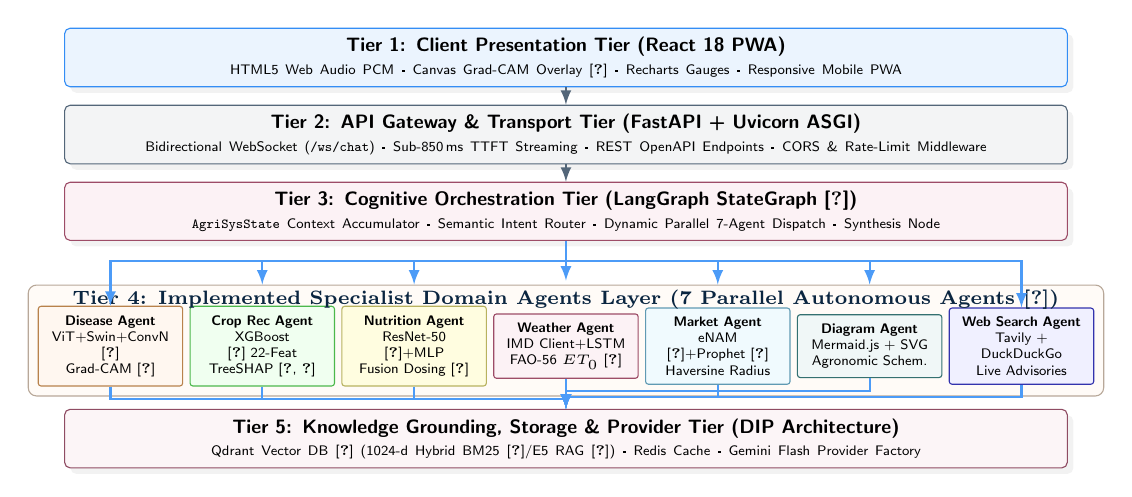
\begin{tikzpicture}[
        node distance=0.22cm and 0.18cm,
        layer/.style={rounded corners=2pt, drop shadow={opacity=0.1}, text width=12.5cm, align=center, font=\scriptsize\sffamily, minimum height=0.52cm},
        agent/.style={rounded corners=1pt, text width=1.60cm, align=center, font=\fontsize{4.8}{5.8}\selectfont\sffamily, minimum height=0.72cm}
    ]
        % T1: Client Presentation Tier
        \node (t1) [layer, draw=secondaryBlue!80, fill=secondaryBlue!8!white] {
            \textbf{Tier 1: Client Presentation Tier (React 18 PWA)} \\
            \tiny HTML5 Web Audio PCM · Canvas Grad-CAM Overlay \cite{gradcam2017} · Recharts Gauges · Responsive Mobile PWA
        };

        % T2: API Gateway Tier
        \node (t2) [layer, below=of t1, draw=primaryBlue!70, fill=primaryBlue!5!white] {
            \textbf{Tier 2: API Gateway \& Transport Tier (FastAPI + Uvicorn ASGI)} \\
            \tiny Bidirectional WebSocket (\texttt{/ws/chat}) · Sub-850\,ms TTFT Streaming · REST OpenAPI Endpoints · CORS \& Rate-Limit Middleware
        };

        % T3: Cognitive Orchestration Tier
        \node (t3) [layer, below=of t2, draw=purple!60!black!70, fill=purple!5!white] {
            \textbf{Tier 3: Cognitive Orchestration Tier (LangGraph StateGraph \cite{langgraph2026})} \\
            \tiny \texttt{AgriSysState} Context Accumulator · Semantic Intent Router · Dynamic Parallel 7-Agent Dispatch · Synthesis Node
        };

        % T4: Specialist Domain Agents (7 Implemented Agents)
        \node (a4) [agent, below=0.92cm of t3, draw=purple!60!black!70, fill=purple!5!white] {\textbf{Weather Agent}\\IMD Client+LSTM\\FAO-56 $ET_0$ \cite{fao56penman1998}};
        \node (a3) [agent, left=0.08cm of a4, draw=yellow!60!black!80, fill=yellow!12!white] {\textbf{Nutrition Agent}\\ResNet-50 \cite{he2016deep}+MLP\\Fusion Dosing \cite{cropibot2026}};
        \node (a2) [agent, left=0.08cm of a3, draw=green!60!black!70, fill=green!6!white] {\textbf{Crop Rec Agent}\\XGBoost \cite{xgboost2016} 22-Feat\\TreeSHAP \cite{shap2017,xaiCrop2024}};
        \node (a1) [agent, left=0.08cm of a2, draw=orange!60!black!70, fill=orange!6!white] {\textbf{Disease Agent}\\ViT+Swin+ConvN \cite{vit2021}\\Grad-CAM \cite{gradcam2017}};
        \node (a5) [agent, right=0.08cm of a4, draw=cyan!60!black!80, fill=cyan!6!white] {\textbf{Market Agent}\\eNAM \cite{enam2023}+Prophet \cite{prophet2018}\\Haversine Radius};
        \node (a6) [agent, right=0.08cm of a5, draw=teal!60!black!80, fill=teal!6!white] {\textbf{Diagram Agent}\\Mermaid.js + SVG\\Agronomic Schem.};
        \node (a7) [agent, right=0.08cm of a6, draw=blue!60!black!80, fill=blue!6!white] {\textbf{Web Search Agent}\\Tavily + DuckDuckGo\\Live Advisories};

        % Container for agents
        \begin{scope}[on background layer]
            \coordinate (a4_top) at ([yshift=0.24cm]a4.north);
            \node[draw=orange!30!black!40, fill=orange!3!white, rounded corners=3pt, inner sep=0.12cm, fit=(a1) (a7) (a4_top)] (agents_container) {};
        \end{scope}
        \node[font=\scriptsize\bfseries\color{primaryBlue}, anchor=north, yshift=0.05cm] (agents_title) at (agents_container.north) {Tier 4: Implemented Specialist Domain Agents Layer (7 Parallel Autonomous Agents \cite{agroaskai2024})};

        % T5: Knowledge, Storage & Provider Tier
        \node (t5) [layer, below=0.38cm of a4, draw=purple!50!black!70, fill=purple!4!white] {
            \textbf{Tier 5: Knowledge Grounding, Storage \& Provider Tier (DIP Architecture)} \\
            \tiny Qdrant Vector DB \cite{qdrant2023} (1024-d Hybrid BM25 \cite{robertson2009probabilistic}/E5 RAG \cite{rag2020}) · Redis Cache · Gemini Flash Provider Factory
        };

        % Connective Arrows
        \draw[-latex, thick, primaryBlue!70] (t1) -- (t2);
        \draw[-latex, thick, primaryBlue!70] (t2) -- (t3);

        % Branching arrows from T3 to agents
        \draw[-latex, thick, secondaryBlue!70] (t3.south) -- +(0,-0.25) -| (a1.north);
        \draw[-latex, thick, secondaryBlue!70] (t3.south) -- +(0,-0.25) -| (agents_container.north -| a2.north);
        \draw[-latex, thick, secondaryBlue!70] (t3.south) -- +(0,-0.25) -| (agents_container.north -| a3.north);
        \draw[-latex, thick, secondaryBlue!70] (t3.south) -- (agents_title.north);
        \draw[-latex, thick, secondaryBlue!70] (t3.south) -- +(0,-0.25) -| (agents_container.north -| a5.north);
        \draw[-latex, thick, secondaryBlue!70] (t3.south) -- +(0,-0.25) -| (agents_container.north -| a6.north);
        \draw[-latex, thick, secondaryBlue!70] (t3.south) -- +(0,-0.25) -| (a7.north);

        % Branching arrows from agents to T5
        \draw[-latex, thick, secondaryBlue!70] (a1.south) -- +(0,-0.16) -| (t5.north);
        \draw[-latex, thick, secondaryBlue!70] (a2.south) -- +(0,-0.16) -| (t5.north);
        \draw[-latex, thick, secondaryBlue!70] (a3.south) -- +(0,-0.16) -| (t5.north);
        \draw[-latex, thick, secondaryBlue!70] (a4.south) -- (t5.north);
        \draw[-latex, thick, secondaryBlue!70] (a5.south) -- +(0,-0.16) -| (t5.north);
        \draw[-latex, thick, secondaryBlue!70] (a6.south) -- +(0,-0.16) -| (t5.north);
        \draw[-latex, thick, secondaryBlue!70] (a7.south) -- +(0,-0.16) -| (t5.north);
    \end{tikzpicture}
\end{frame}

% =========================================================================
% CONTENT SLIDE 6: IMPLEMENTATION PROGRESS - PART 1
% (Core Cognitive Orchestration, Vision Diagnostics & Grounded RAG)
% =========================================================================
\section{Implementation Progress}
\begin{frame}{Core AI \& Diagnostics}
    \vspace{-0.3cm}
    \begin{columns}[T,onlytextwidth]
        \begin{column}{0.50\textwidth}
            \fontsize{5.8}{6.8}\selectfont
            \stagelabel{\color{primaryBlue}Stage 1 \textbf{\textperiodcentered} DIP Provider \& Hybrid Knowledge RAG}{primaryBlue!10}{primaryBlue!40}
            \begin{itemize}\setlength{\itemsep}{0.6pt}\setlength{\parsep}{0pt}\setlength{\topsep}{1pt}
                \item \textbf{DIP Factory:} Pluggable backend --- Gemini 3.8 Flash, GPT-4o, Groq Llama-3.3-70B, Ollama.
                \item \textbf{Hybrid RAG \cite{rag2020}:} Qdrant \cite{qdrant2023} 1024-d (e5-large) + BM25 \cite{robertson2009probabilistic} $\to$ RRF ($k\!=\!60$) \cite{cormack2009reciprocal} over 250k+ ICAR chunks \cite{ragMaize2026}.
                \item \textbf{Guard:} Cross-Encoder \cite{reimers2019sentence} + HallucinationGuard ($\ge\!0.70$) \cite{ragas2023}. \textbf{0.884 MRR@5, 93.6\% Hit-Rate.}
            \end{itemize}
            \vspace{2pt}
            \stagelabel{\color{orange!80!black}Stage 2 \textbf{\textperiodcentered} Vision Pathology \& Grad-CAM XAI}{orange!10}{orange!50}
            \begin{itemize}\setlength{\itemsep}{0.6pt}\setlength{\parsep}{0pt}\setlength{\topsep}{1pt}
                \item \textbf{Ensemble:} ViT-B/16 \cite{vit2021} + Swin-T \cite{swinTransformer2021} + ConvNeXt-Tiny \cite{convnext2022}; BRISQUE \cite{mittal2012no} QA ($\le\!45$) + CLAHE.
                \item \textbf{XAI:} Grad-CAM \cite{gradcam2017} overlays with severity [0--5]. \textbf{94.2\% Top-1 Acc, 0.93 Macro-F1.}
            \end{itemize}
            \vspace{2pt}
            \stagelabel{\color{green!70!black}Stage 3 \textbf{\textperiodcentered} LangGraph Orchestrator \& Crop Recommender}{green!8}{green!50}
            \begin{itemize}\setlength{\itemsep}{0.6pt}\setlength{\parsep}{0pt}\setlength{\topsep}{1pt}
                \item \textbf{StateGraph \cite{langgraph2026}:} 7-class intent router $\to$ \texttt{AgriSysState} typed-dict \cite{agroaskai2024} + parallel \texttt{ResponseMerger}.
                \item \textbf{Crop ML:} 22-feature XGBoost \cite{xgboost2016} / RF \textbf{(95.8\% Acc)} + TreeSHAP \cite{shap2017,xaiCrop2024} what-if simulator.
            \end{itemize}
            \vspace{2pt}
            \stagelabel{\color{yellow!60!black}Stage 4 \textbf{\textperiodcentered} Cross-Modal Soil Nutrition Fusion}{yellow!10}{yellow!60!black!40}
            \begin{itemize}\setlength{\itemsep}{0.6pt}\setlength{\parsep}{0pt}\setlength{\topsep}{1pt}
                \item ResNet-50 \cite{he2016deep} image features + 7-channel IoT telemetry (N, P, K, pH, EC, temp, moisture) $\to$ MLP $\to$ ICAR SHC fertilizer dosage (kg/ha) \cite{cropibot2026}.
            \end{itemize}
        \end{column}

        \begin{column}{0.48\textwidth}
            \vspace{-0.10cm}
            \centering
            {\fontsize{7}{8}\selectfont\bfseries\color{primaryBlue} Cognitive Diagnostic \& RAG Dataflow}\\[2pt]
            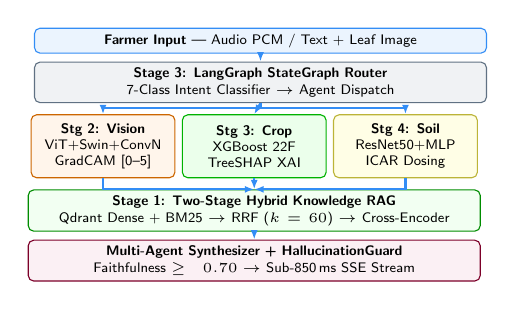
\begin{tikzpicture}[
                node distance=0.10cm,
                flow/.style={rounded corners=2pt, draw=primaryBlue!65, fill=white, text width=5.6cm, align=center, font=\fontsize{5.3}{6.2}\selectfont\sffamily, inner sep=2pt},
                agentb/.style={rounded corners=2pt, text width=1.70cm, align=center, font=\fontsize{4.8}{5.8}\selectfont\sffamily, inner sep=1.8pt, minimum height=0.80cm},
                arrow/.style={-{Latex[length=1.2mm,width=0.9mm]}, thick, secondaryBlue!80}
            ]
                \node[flow, draw=secondaryBlue!80, fill=secondaryBlue!8] (inp)
                    {\textbf{Farmer Input} --- Audio PCM / Text + Leaf Image};
                \node[flow, below=0.10cm of inp, fill=primaryBlue!6] (router)
                    {\textbf{Stage 3: LangGraph StateGraph Router}\\7-Class Intent Classifier $\to$ Agent Dispatch};

                \node[agentb, below=0.14cm of router, xshift=-2.0cm, draw=orange!80!black, fill=orange!8] (ag_dis)
                    {\textbf{Stg 2: Vision}\\ViT+Swin+ConvN\\GradCAM [0--5]};
                \node[agentb, right=0.08cm of ag_dis, draw=green!70!black, fill=green!8] (ag_crp)
                    {\textbf{Stg 3: Crop}\\XGBoost 22F\\TreeSHAP XAI};
                \node[agentb, right=0.08cm of ag_crp, draw=yellow!70!black, fill=yellow!10] (ag_nut)
                    {\textbf{Stg 4: Soil}\\ResNet50+MLP\\ICAR Dosing};

                \node[flow, below=0.14cm of ag_crp, draw=green!55!black, fill=green!5] (rag)
                    {\textbf{Stage 1: Two-Stage Hybrid Knowledge RAG}\\Qdrant Dense + BM25 $\to$ RRF ($k\!=\!60$) $\to$ Cross-Encoder};

                \node[flow, below=0.10cm of rag, draw=purple!65!black, fill=purple!6] (merger)
                    {\textbf{Multi-Agent Synthesizer + HallucinationGuard}\\Faithfulness $\ge 0.70$ $\to$ Sub-850\,ms SSE Stream};

                \draw[arrow] (inp) -- (router);
                \draw[arrow] (router.south) -- +(0,-0.06) -| (ag_dis.north);
                \draw[arrow] (router.south) -- (ag_crp.north);
                \draw[arrow] (router.south) -- +(0,-0.06) -| (ag_nut.north);
                \draw[arrow] (ag_dis.south) |- (rag.north);
                \draw[arrow] (ag_crp.south) -- (rag.north);
                \draw[arrow] (ag_nut.south) |- (rag.north);
                \draw[arrow] (rag) -- (merger);
            \end{tikzpicture}
        \end{column}
    \end{columns}
\end{frame}

% =========================================================================
% CONTENT SLIDE 7: IMPLEMENTATION PROGRESS - PART 2
% (Market Intelligence, Voice, PWA & Production Microservices)
% =========================================================================
\begin{frame}{Market, Voice \& Production}
    \vspace{-0.3cm}
    \begin{columns}[T,onlytextwidth]
        \begin{column}{0.50\textwidth}
            \fontsize{5.8}{6.8}\selectfont
            \stagelabel{\color{primaryBlue}Stage 5 \textbf{\textperiodcentered} Market Intelligence \& Mandi Forecasting}{primaryBlue!8}{primaryBlue!40}
            \begin{itemize}\setlength{\itemsep}{0.6pt}\setlength{\parsep}{0pt}\setlength{\topsep}{1pt}
                \item \textbf{APMC Ingestion:} Live Agmarknet \cite{enam2023} client, 2,500+ mandis; Haversine spatial rank within 50\,km.
                \item \textbf{Forecasting:} Prophet \cite{prophet2018} 7-day commodity price model \textbf{(8.4\% MAPE)} + MSP arbitrage advisory.
            \end{itemize}
            \vspace{2pt}
            \stagelabel{\color{blue!70!black}Stage 6 \textbf{\textperiodcentered} Meteorological \& Hydrology Advisory}{blue!6}{blue!40}
            \begin{itemize}\setlength{\itemsep}{0.6pt}\setlength{\parsep}{0pt}\setlength{\topsep}{1pt}
                \item \textbf{$\mathrm{ET}_0$ Model:} FAO-56 Penman-Monteith \cite{fao56penman1998} irrigation schedule + IMD gridded telemetry integration.
                \item \textbf{Hazard Alerts:} Bi-LSTM classifier for frost, drought, and heavy precipitation anomalies.
            \end{itemize}
            \vspace{2pt}
            \stagelabel{\color{purple!80!black}Stage 7 \textbf{\textperiodcentered} End-to-End Indic Voice Pipeline}{purple!6}{purple!40}
            \begin{itemize}\setlength{\itemsep}{0.6pt}\setlength{\parsep}{0pt}\setlength{\topsep}{1pt}
                \item Whisper Large-v3 \cite{whisper2022} streaming ASR + Silero VAD $\to$ \textbf{14.8\% Hindi WER} \cite{indicAsr2025}.
                \item Bhashini \cite{bhashini2023} Indic TTS ($<\!650$\,ms) + text normalizer for 10 Indian regional languages.
            \end{itemize}
            \vspace{2pt}
            \stagelabel{\color{secondaryBlue!80!black}Stage 8 \textbf{\textperiodcentered} React 18 Full-Stack Progressive Web App}{secondaryBlue!8}{secondaryBlue!50}
            \begin{itemize}\setlength{\itemsep}{0.6pt}\setlength{\parsep}{0pt}\setlength{\topsep}{1pt}
                \item Vite 5 PWA: WebSocket token-streaming, Voice Studio PCM visualizer, Grad-CAM canvas overlay, SHC sliders.
                \item Offline-capable Service Workers + sub-850\,ms TTFT first-token delivery.
            \end{itemize}
        \end{column}

        \begin{column}{0.48\textwidth}
            \vspace{-0.10cm}
            \centering
            {\fontsize{7}{8}\selectfont\bfseries\color{primaryBlue} Production Architecture \& Verified Milestones}\\[2pt]
            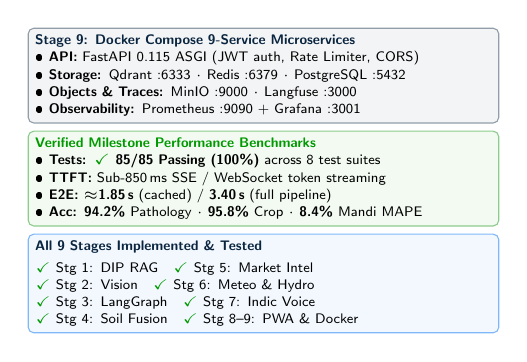
\begin{tikzpicture}[
                box/.style={rounded corners=2pt, draw=primaryBlue!45, fill=white, text width=5.8cm, font=\fontsize{5.3}{6.2}\selectfont\sffamily, inner sep=2.5pt}
            ]
                \node[box, fill=primaryBlue!5] (topo) {
                    \textbf{\color{primaryBlue}Stage 9: Docker Compose 9-Service Microservices}\\
                    \textbullet\ \textbf{API:} FastAPI 0.115 ASGI (JWT auth, Rate Limiter, CORS)\\
                    \textbullet\ \textbf{Storage:} Qdrant :6333 $\cdot$ Redis :6379 $\cdot$ PostgreSQL :5432\\
                    \textbullet\ \textbf{Objects \& Traces:} MinIO :9000 $\cdot$ Langfuse :3000\\
                    \textbullet\ \textbf{Observability:} Prometheus :9090 + Grafana :3001
                };

                \node[box, below=0.09cm of topo, fill=green!60!black!5, draw=green!55!black!45] (bench) {
                    \textbf{\color{green!60!black}Verified Milestone Performance Benchmarks}\\
                    \textbullet\ \textbf{Tests:} {\color{green!60!black}\checkmark} \textbf{85/85 Passing (100\%)} across 8 test suites\\
                    \textbullet\ \textbf{TTFT:} Sub-850\,ms SSE / WebSocket token streaming\\
                    \textbullet\ \textbf{E2E:} $\approx$\textbf{1.85\,s} (cached) / \textbf{3.40\,s} (full pipeline)\\
                    \textbullet\ \textbf{Acc:} \textbf{94.2\%} Pathology $\cdot$ \textbf{95.8\%} Crop $\cdot$ \textbf{8.4\%} Mandi MAPE
                };

                \node[box, below=0.09cm of bench, fill=secondaryBlue!5, draw=secondaryBlue!50] (status) {
                    \textbf{\color{primaryBlue}All 9 Stages Implemented \& Tested}\\[2pt]
                    {\fontsize{5.0}{6.0}\selectfont\sffamily
                    {\color{green!60!black}\checkmark} Stg 1: DIP RAG\quad
                    {\color{green!60!black}\checkmark} Stg 5: Market Intel\\
                    {\color{green!60!black}\checkmark} Stg 2: Vision\quad
                    {\color{green!60!black}\checkmark} Stg 6: Meteo \& Hydro\\
                    {\color{green!60!black}\checkmark} Stg 3: LangGraph\quad
                    {\color{green!60!black}\checkmark} Stg 7: Indic Voice\\
                    {\color{green!60!black}\checkmark} Stg 4: Soil Fusion\quad
                    {\color{green!60!black}\checkmark} Stg 8--9: PWA \& Docker}
                };
            \end{tikzpicture}
        \end{column}
    \end{columns}
\end{frame}

% =========================================================================
% CONTENT SLIDE 8: FUTURE WORK & COMPLETION ROADMAP
% =========================================================================
\section{Future Work \& Roadmap}
\begin{frame}{Future Work \& Technical Roadmap}
    \begin{columns}[T]
        \begin{column}{0.52\textwidth}
            \textbf{\small Upcoming Milestones \& Onboarding Work}
            \begin{itemize}\small\setlength{\itemsep}{2pt}
                \item \textbf{Data Collection for RAG:} Curate regional agronomic documents, KVK advisories, and local soil/crop datasets \cite{ragMaize2026,rag2020}.
                \item \textbf{Video Model Integration:} Add temporal models to track pest mobility and lesion progression \cite{agronvila2026,deeplearning2025}.
                \item \textbf{Edge \& Optimization:} INT8/ONNX Runtime distillation \cite{onnx2019} for offline edge inference and token streaming.
                \item \textbf{Setup, Debugging \& Onboarding:} Multi-container orchestration, async queue tuning, WebSocket stability.
                \item \textbf{Final Evaluation:} RAGAS \cite{ragas2023} and MIRAGE \cite{mirage2025}/AgMMU \cite{agmmu2025} benchmarks.
            \end{itemize}
        \end{column}
        \begin{column}{0.44\textwidth}
            \textbf{\small Delivery Schedule}
            \renewcommand{\arraystretch}{1.0}
            \resizebox{\linewidth}{!}{
                \begin{tabular}{lll}
                    \toprule
                    \textbf{Period} & \textbf{Milestone Focus} & \textbf{Status} \\
                    \midrule
                    M1--3 & RAG Architecture \& Corpus Setup \cite{rag2020} & \ok{Completed} \\
                    M4--6 & Agent Models \& Indic Voice Pipeline \cite{whisper2022} & \ok{Completed} \\
                    M7--8 & Web PWA UI \& Gateway Integration & \ok{Completed} \\
                    \rowcolor{secondaryBlue!10} \textbf{M9} & \textbf{Multi-Agent Engine \& Tool Setup} & \ok{\textbf{Current}} \\
                    M10 & Corpus Expansion \& Video Model Integration & In Progress \\
                    M11 & Edge Optimization \& System Debugging \cite{onnx2019} & Upcoming \\
                    M12 & Final Benchmark Evaluation \cite{ragas2023,mirage2025} & Target \\
                    \bottomrule
                \end{tabular}
            }
            \begin{itemize}\small\setlength{\itemsep}{1pt}
                \item \textbf{Key Contribution:} First 7-agent system with explainable diagnostics \cite{gradcam2017,shap2017}, sensor fusion \cite{cropibot2026}, and Indic voice \cite{indicAsr2025,bhashini2023}.
            \end{itemize}
        \end{column}
    \end{columns}
\end{frame}

% =========================================================================
% REFERENCES
% =========================================================================
\section{References}
\begin{frame}[allowframebreaks]{References}
    \tiny
    \setbeamertemplate{bibliography item}[text]
    \bibliographystyle{abbrv}
    
    \let\oldthebibliography\thebibliography
    \let\endoldthebibliography\endthebibliography
    \renewenvironment{thebibliography}[1]{%
        \begin{oldthebibliography}{#1}%
        \setlength{\itemsep}{0pt}%
        \setlength{\parsep}{0pt}%
    }{%
        \end{oldthebibliography}%
    }
    
    \bibliography{references}
\end{frame}

% =========================================================================
% THANK YOU FRAME
% =========================================================================
\begin{frame}[plain]
    \begin{tikzpicture}[remember picture,overlay]
        % Dark Navy full page background
        \fill[primaryBlue] (current page.south west) rectangle (current page.north east);
        
        % Geometric accent shapes matching the title page theme
        \path[fill=secondaryBlue, opacity=0.7] (current page.south west) -- ([xshift=0.4\paperwidth]current page.south west) -- ([xshift=0.2\paperwidth]current page.north west) -- cycle;
        \path[fill=accentGold, opacity=0.8] (current page.north east) -- ([xshift=-0.3\paperwidth]current page.north east) -- ([xshift=-0.15\paperwidth]current page.south east) -- cycle;
        
        % Small logo in top left
        \node[anchor=north west, xshift=1.2cm, yshift=-0.6cm] at (current page.north west) {
            
\includegraphics[height=1.2cm]{Logo_IIITL.png}
        };
        
        % Centered Thank You content
        \node[anchor=center, align=center, text width=0.7\paperwidth] at (current page.center) {
            {\color{white}\Huge\bfseries Thank You!}\par
            \vspace{0.4cm}
            {\color{accentGold}\Large\bfseries Questions \& Discussion}\par
            \vspace{0.8cm}
            {\color{white!90}\large\bfseries Shajid Ali Khan}\par
            \vspace{0.15cm}
            {\color{white!70}\small Department of Computer Science \\ Indian Institute of Information Technology, Lucknow}\par
            \vspace{0.4cm}
            {\color{secondaryBlue!40}\footnotesize\ttfamily mcs25049@iiitl.ac.in}
        };
    \end{tikzpicture}
\end{frame}

\end{document}
